\documentclass[conference]{IEEEtran}
\usepackage{cite}
\usepackage{amsmath,amssymb,amsfonts}
\usepackage{array}
\usepackage{booktabs}
\usepackage{multirow}
\usepackage{xcolor}
\usepackage{url}
\usepackage{enumitem}
\usepackage{tikz}
\usetikzlibrary{arrows.meta,positioning,shapes.geometric}

\newcommand{\model}{\mathcal{M}}
\newcommand{\coverage}{\mathcal{C}}
\newcommand{\ind}{\mathbb{1}}

\begin{document}

\title{How Many Dimensions Are There in Space? DimensionBridge: A Cross-Scale Falsifiability Design for Extra-Dimension Models}

\author{\IEEEauthorblockN{Research Proposal Generated from a Four-Agent Evidence-to-Design Workflow}
\IEEEauthorblockA{Survey $\rightarrow$ Idea $\rightarrow$ ExperimentDesign $\rightarrow$ Author\\
Theoretical physics, precision gravity, collider phenomenology, and gravitational-wave inference}}

\maketitle

\begin{abstract}
We observe three extended spatial dimensions, but this fact does not determine the dimensionality of a fundamental theory. Extra dimensions may be compact, warped, inaccessible to standard-model fields, or expressed only through model-dependent modifications of gravitational or particle phenomenology. This paper develops DimensionBridge, a design-only cross-scale falsifiability atlas for extra-dimension models. Rather than attempting to measure a universal ``number of dimensions,'' the framework records a model class, parameter domain, low-energy translation, channel-specific observable, likelihood assumptions, competing explanations, and an auditable model status. It connects short-range gravity, collider missing-momentum or resonance searches, gravitational-wave propagation, and cosmological/astrophysical constraints only when their parameter conventions and independence conditions permit combination. The output categories are excluded within assumptions, currently compatible, sensitivity-limited, observationally unidentifiable, and requires independent test. Three testable propositions concern translation discipline, cross-channel complementarity, and anomaly attribution. The proposal reports no new measurement, no detector reanalysis, and no empirical discovery. Its contribution is a rigorous way to say what existing and future observations can, and cannot, establish about extra spatial dimensions.
\end{abstract}

\begin{IEEEkeywords}
extra dimensions, string theory, Kaluza--Klein theory, short-range gravity, collider phenomenology, gravitational waves, model selection, falsifiability
\end{IEEEkeywords}

\section{Introduction}

Space appears to have three extended dimensions: length, width, and height. Together with time, these coordinates organize every ordinary laboratory measurement and the four-dimensional effective description used by general relativity and the Standard Model. This observation is sometimes placed beside a very different statement: perturbative superstring theories are naturally formulated in ten spacetime dimensions, and an eleven-dimensional limit is associated with M-theory \cite{polchinski,witten}. The juxtaposition can make ``How many dimensions are there?'' sound like a question with a single numerical answer awaiting an experiment.

It is not. A spacetime dimension can be extended or compact; it can support only gravity or also other fields; it can be flat or warped; and it can affect accessible physics through a force law, a particle spectrum, a production rate, a propagation law, or not at all in an accessible regime. The number in a formal construction therefore is not automatically a direct observable. Conversely, a laboratory or astrophysical null result constrains an analysis model, parameter domain, and systematic treatment; it does not prove that every higher-dimensional completion has been ruled out.

This paper proposes \textbf{DimensionBridge}, an evidence-to-decision framework for preserving these distinctions. The target is not a universal dimension count. The target is a falsifiability map: which extra-dimension model classes produce distinguishable signals in which channels, under which assumptions, and with what conditions for exclusion, compatibility, non-identifiability, or independent replication.

The proposal is the Author-stage result of a four-agent workflow. The Survey stage constructed a source-bound evidence boundary and research-gap ledger. The Idea stage compared a parameter registry, single-channel extensions, a cross-scale atlas, and a speculative compactification score; it selected the atlas. The ExperimentDesign stage converted that direction into a computational synthesis and likelihood-translation plan. This paper organizes those artifacts as an IEEE-style research proposal. It does not report a new torsion-balance measurement, collider analysis, gravitational-wave catalog reanalysis, cosmological inference, or extra-dimension discovery.

\section{Evidence Boundary and Research Gap}

\subsection{Observed dimensions, formal dimensions, and effective dimensions}

The operationally established statement is modest and strong: at presently accessible macroscopic and microscopic scales, physical observations are well described by three extended spatial directions and one time direction. A dimension count beyond this baseline requires a physical model that links hidden structure to an observable departure from four-dimensional effective physics.

Kaluza--Klein reasoning provides the canonical illustration. A compact spatial direction can be invisible to low-energy position measurements while inducing a tower of modes or effective fields after dimensional reduction. String theory provides another motivation: consistent perturbative superstrings live in ten spacetime dimensions, while Witten's strong-coupling argument connects several string theories to an eleven-dimensional description \cite{polchinski,witten}. Neither result says that a detector must reveal six or seven additional spatial directions at a fixed accessible scale. The outcome depends on compactification, moduli, branes, stabilization, supersymmetry breaking, and the low-energy spectrum.

Two influential effective scenarios make the gap from formal dimension to observability explicit. In ADD models, several flat compact dimensions can lower the fundamental gravity scale relative to the observed four-dimensional Planck scale \cite{add}. In RS models, a warped fifth direction reshapes the relation between scales and can create distinct localization or Kaluza--Klein phenomenology \cite{rs1,rs2}. These models do not predict the same signatures and must not be placed into one unqualified ``extra dimensions'' likelihood.

\subsection{Four complementary observational routes}

Short-range gravity experiments search for departures from Newtonian behavior at small separations. A common phenomenological form is

\begin{equation}
V(r)=-\frac{Gm_1m_2}{r}\left[1+\alpha\exp\left(-\frac{r}{\lambda}\right)\right],
\label{eq:yukawa}
\end{equation}

where $\alpha$ is a relative interaction strength and $\lambda$ is its range. Equation~\eqref{eq:yukawa} is experimentally useful because it converts a force measurement into a likelihood over $(\alpha,\lambda)$. It is not the universal law of extra dimensions. The translation to a compactification radius, number of dimensions, or brane coupling depends on the model. Recent torsion-balance work improves bounded regions of such non-Newtonian parameter space \cite{lee2020}; the scientific interpretation must retain the translation conditions.

Collider searches can probe high-energy versions of the same broad theoretical territory. In ADD-like theories, inaccessible Kaluza--Klein excitations may appear as missing transverse momentum, while warped models can motivate resonances or other structures. ATLAS and CMS analyses publish limits under explicit signal, effective-field-theory, and detector assumptions \cite{atlas2021,cms2019}. Their strength is high energy and controlled event reconstruction; their limitation is that a reported mass-scale bound is conditional on the analysis model and treatment of ultraviolet validity.

Gravitational-wave observations add a long-baseline propagation channel. A crossover to higher-dimensional propagation can alter amplitude damping or other distance relations, as proposed for standard-siren tests \cite{deffayet2007}. General-relativity tests using compact-binary catalogs constrain specified propagation deviations \cite{abbott2019}. But nonstandard damping can also arise from calibration, source-population, cosmological, or modified-gravity effects not uniquely tied to an extra dimension. A gravitational-wave residual should therefore trigger a competing-model test, not a direct dimension count.

Astrophysical and cosmological arguments can reach parameter ranges inaccessible to laboratories, but they introduce their own history-dependent assumptions. For example, energy-loss reasoning in compact objects constrains selected large-extra-dimension scenarios while relying on astrophysical modeling and the chosen bulk spectrum \cite{hannestad2003}. Complementarity is valuable precisely because the channels do not share the same approximations; it becomes misleading when they are combined without recording their differing assumptions.

\subsection{Research gaps}

The central gap is not the absence of clever experiments. It is an inference problem. A cross-scale literature often contains individual limits, forecast curves, and theory constructions without an auditable connection between them. Table~\ref{tab:gaps} records the gaps carried from the Survey stage.

\begin{table*}[t]
\caption{Evidence-derived gaps and the corresponding DimensionBridge response.}
\label{tab:gaps}
\centering
\footnotesize
\setlength{\tabcolsep}{3pt}
\begin{tabular}{p{0.08\textwidth} p{0.39\textwidth} p{0.43\textwidth}}
\toprule
\textbf{ID} & \textbf{Gap} & \textbf{DimensionBridge response} \\
\midrule
G1 & Observed spatial dimensions, formal string-theory dimensions, compactification, and modified-gravity phenomenology are commonly conflated. & Require every claim to begin with a model class and accessible scale. \\
G2 & Experimental limits are often detached from compactification, warping, coupling, and EFT-validity assumptions. & Attach a translation card to each source likelihood or limit. \\
G3 & Laboratory, collider, GW, and cosmological information lack a common, auditable complementarity structure. & Build a parameter-coverage and overlap atlas before likelihood combination. \\
G4 & Null results are overstated as global no-go theorems; formal consistency is overstated as empirical confirmation. & Report bounded status categories rather than a yes/no answer. \\
G5 & Candidate anomalies lack a shared alternative-explanation and replication rule. & Require competing-model, systematic, and independent-channel matrices. \\
G6 & Compatibility with current data is confused with empirical support when no accessible observable exists. & Use an explicit observational-identifiability audit. \\
\bottomrule
\end{tabular}
\end{table*}

\section{DimensionBridge Hypothesis and Architecture}

\subsection{Testable propositions}

DimensionBridge makes three propositions that can be evaluated by a preregistered case-study set.

\begin{itemize}[leftmargin=*,nosep]
\item \textbf{H1 -- Translation discipline:} a limit changes a model status only where a source-bound model-to-observable map covers the relevant parameter region. The framework should prevent isolated null results from becoming false global exclusions.
\item \textbf{H2 -- Complementarity discipline:} jointly using genuinely compatible and independent channels should improve classification of selected parameter regions over any single channel, without manufacturing precision from duplicated information.
\item \textbf{H3 -- Discovery discipline:} a putative excess remains a requirement for independent testing until it survives a preregistered alternative-explanation and replication matrix.
\end{itemize}

These are scientific claims about an inference architecture, not claims that higher dimensions have been detected. H1 fails if removal of a compactification or EFT assumption leaves a numerical exclusion unchanged. H2 fails if a joint result depends on incompatible conventions, correlated data treated as independent, or prior-volume artifacts. H3 fails if the framework uniquely attributes a generic force, resonance, or propagation deviation to extra dimensions without discriminating observables.

\subsection{Architecture}

Fig.~\ref{fig:bridge} shows the chain of custody for an inference. A model class is paired with parameter and assumption cards, translated into channel-specific predictions, tested for likelihood-combination compatibility and competing explanations, and finally routed into a status. The status is not an award of truth. `CURRENTLY COMPATIBLE` means current data do not exclude the declared region. `OBSERVATIONALLY UNIDENTIFIABLE` means that no valid accessible observable map is available; it must not be promoted to support.

\begin{figure*}[t]
\centering
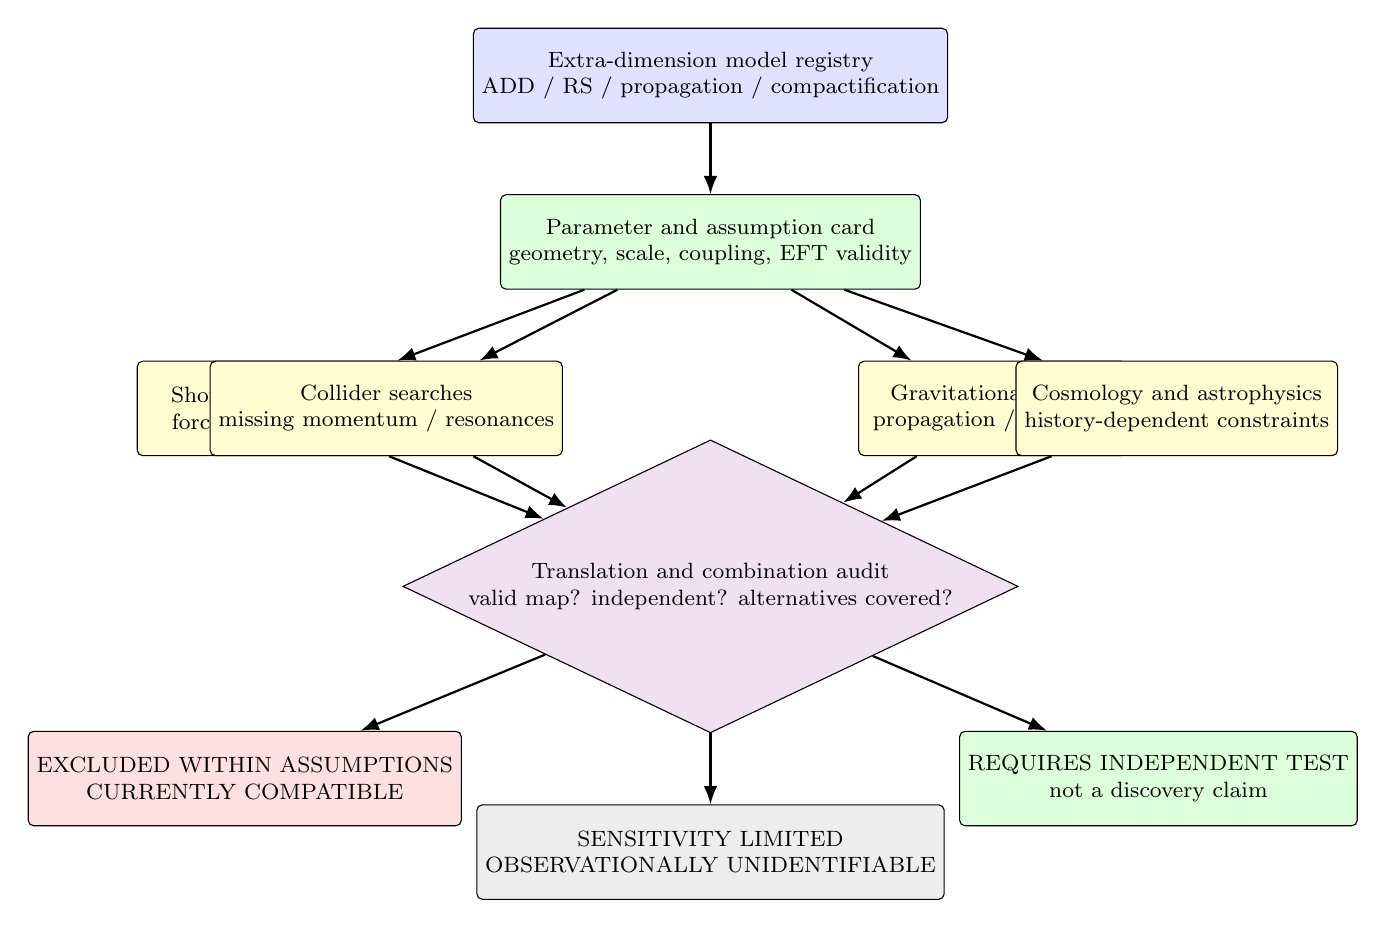
\begin{tikzpicture}[font=\footnotesize, node distance=9mm and 12mm, >=Latex,
 box/.style={draw, rounded corners=2pt, align=center, minimum width=34mm, minimum height=12mm, inner sep=3pt},
 decision/.style={draw, diamond, aspect=2.1, align=center, inner sep=2pt, minimum width=37mm, minimum height=12mm},
 line/.style={->, thick}]
\node[box, fill=blue!12] (model) {Extra-dimension model registry\\ADD / RS / propagation / compactification};
\node[box, fill=green!14, below=of model] (param) {Parameter and assumption card\\geometry, scale, coupling, EFT validity};
\node[box, fill=yellow!18, below left=of param] (grav) {Short-range gravity\\force-law likelihood};
\node[box, fill=yellow!18, below left=of param, xshift=20mm] (collider) {Collider searches\\missing momentum / resonances};
\node[box, fill=yellow!18, below right=of param, xshift=-20mm] (gw) {Gravitational waves\\propagation / damping};
\node[box, fill=yellow!18, below right=of param] (cosmo) {Cosmology and astrophysics\\history-dependent constraints};
\node[decision, fill=violet!12, below=19mm of param] (audit) {Translation and combination audit\\valid map? independent? alternatives covered?};
\node[box, fill=red!12, below left=of audit] (status1) {EXCLUDED WITHIN ASSUMPTIONS\\CURRENTLY COMPATIBLE};
\node[box, fill=gray!14, below=of audit] (status2) {SENSITIVITY LIMITED\\OBSERVATIONALLY UNIDENTIFIABLE};
\node[box, fill=green!14, below right=of audit] (status3) {REQUIRES INDEPENDENT TEST\\not a discovery claim};
\draw[line] (model)--(param);
\draw[line] (param)--(grav); \draw[line] (param)--(collider); \draw[line] (param)--(gw); \draw[line] (param)--(cosmo);
\draw[line] (grav)--(audit); \draw[line] (collider)--(audit); \draw[line] (gw)--(audit); \draw[line] (cosmo)--(audit);
\draw[line] (audit)--(status1); \draw[line] (audit)--(status2); \draw[line] (audit)--(status3);
\end{tikzpicture}
\caption{DimensionBridge chain from theory statement to bounded model status. The editable source is supplied as \texttt{figures/dimensionbridge\_architecture.drawio}. A channel enters joint inference only after translation, independence, and alternative-explanation checks.}
\label{fig:bridge}
\end{figure*}

\subsection{Formal combination rule}

Let $\model$ denote a model class, $\theta$ its physical parameters, $O_c$ the observation from channel $c$, $f_c(\model,\theta)$ the declared prediction map, and $\eta_c$ channel-specific nuisance parameters. The planned joint object is

\begin{equation}
\mathcal{L}_{\mathrm{joint}}(\model,\theta)=
\prod_{c\in\mathcal{K}(\model,\theta)}
\mathcal{L}_c\left[O_c\mid f_c(\model,\theta),\eta_c\right].
\label{eq:joint}
\end{equation}

The set $\mathcal{K}$ is intentionally restricted. A channel can appear in Eq.~\eqref{eq:joint} only if its units, parameter convention, likelihood construction, validity assumptions, and dependence with other channels are documented as compatible. Equation~\eqref{eq:joint} is a future analysis structure; this report does not calculate it from data.

Before any combination, the atlas computes an interpretable coverage quantity,

\begin{equation}
\coverage(\model,\theta)=\sum_c w_c\ind_c(\model,\theta),
\label{eq:coverage}
\end{equation}

where $\ind_c=1$ only if channel $c$ possesses a valid observable map and declared sensitivity at the point $(\model,\theta)$. The weight $w_c$ records methodological independence and robustness; it is not a subjective vote for the theory. A parameter region with low $\coverage$ is not protected from criticism, but it must be reported as sensitivity-limited or observationally unidentifiable rather than as supported.

\section{Design-Only Methods}

\subsection{Model registry and source cards}

The study begins with model classes, not experiments. Table~\ref{tab:models} defines the planned registry. The purpose is not to exhaust every string compactification. It is to include representative model-to-observable chains whose distinctions matter for inference.

\begin{table*}[t]
\caption{Planned model registry and required translation evidence.}
\label{tab:models}
\centering
\footnotesize
\setlength{\tabcolsep}{2.7pt}
\begin{tabular}{p{0.13\textwidth} p{0.25\textwidth} p{0.27\textwidth} p{0.25\textwidth}}
\toprule
\textbf{Class} & \textbf{Parameters to register} & \textbf{Accessible observables} & \textbf{Translation risk} \\
\midrule
M0: 4D baseline & GR/SM nuisance and systematic parameters. & Force, collider, GW, and cosmology baseline likelihoods. & Baseline systematics can mimic a small anomaly. \\
M1: ADD-like flat compact dimensions & Number of dimensions, compactification scale/radius, fundamental gravity scale, EFT cutoff. & Yukawa-like deviations, missing momentum, astrophysical energy loss. & EFT truncation and bulk-state assumptions. \\
M2: RS-like warped dimension & Warp scale, curvature ratio, brane localization, resonance couplings. & Resonance and nonresonant collider signatures; precision constraints. & Spectrum and coupling conventions. \\
M3: altered propagation ansatz & Crossover scale, damping/dispersion parameter, dimensional-flow form. & GW amplitude/distance and multi-messenger propagation. & Degeneracy with cosmology, calibration, and non-extra-dimensional modified gravity. \\
M4: formal compactification class & Geometry, moduli, stabilization, low-energy spectrum. & Only a concrete derived effective observable, if available. & May be observationally unidentifiable at accessible scales. \\
\bottomrule
\end{tabular}
\end{table*}

For every published input, a source card stores the experimental or theoretical source identifier, observable definition, model class, parameter units, confidence construction, nuisance treatment, selection or calibration assumptions, and provenance. A separate translation card stores the logical path from the source likelihood to a model parameter. The translation card has five nonmergeable fields: directly fitted observable; derived prediction; compactification/warping/UV prior; alternative explanation; and unknown region. This is the design's main defense against accidental overstatement.

\subsection{Channel eligibility and alternative explanations}

The potential channels have different inferential roles (Table~\ref{tab:channels}). A short-range force experiment may have a clean geometry but limited reach in scale. A collider analysis may reach high energy but depend on a signal model and event-selection interpretation. Gravitational-wave propagation has a long lever arm but shares degeneracies with source and cosmology modeling. Cosmological arguments can be sensitive to bulk effects while depending on assumptions about cosmic history. Treating them as interchangeable constraints would reduce, rather than improve, rigor.

\begin{table*}[t]
\caption{Channel eligibility criteria and non-extra-dimensional alternatives.}
\label{tab:channels}
\centering
\footnotesize
\setlength{\tabcolsep}{2.7pt}
\begin{tabular}{p{0.16\textwidth} p{0.28\textwidth} p{0.25\textwidth} p{0.22\textwidth}}
\toprule
\textbf{Channel} & \textbf{Eligible input} & \textbf{Required alternatives} & \textbf{Combination condition} \\
\midrule
Short-range gravity & Published force/residual likelihood with separation, geometry, and calibration treatment. & Scalar fifth force, electromagnetic backgrounds, mass-distribution error. & Shared Yukawa or model parameter convention is explicit. \\
Collider & Public limit/likelihood with signal model, acceptance, uncertainty, and EFT treatment. & SM background mismodeling, ordinary resonance, dark-sector or other BSM signatures. & Analysis regions are independent or correlations are modeled. \\
Gravitational waves & Propagation likelihood with waveform, calibration, source-population, and cosmology assumptions. & Calibration bias, lensing, population evolution, modified gravity without extra dimensions. & Distance/redshift and propagation parameter definitions agree. \\
Cosmology/astrophysics & Bound with thermal history, stellar/compact-object, and particle-content assumptions. & Astrophysical modeling, hidden-sector physics, uncertain history. & No contradictory thermal or spectrum assumptions are silently pooled. \\
\bottomrule
\end{tabular}
\end{table*}

The study includes an alternative-explanation matrix. An anomaly can progress toward `REQUIRES INDEPENDENT TEST` only if its expected behavior differs from at least one viable alternative in a future public observable. Without that discriminator, the appropriate status is `OBSERVATIONALLY\_UNIDENTIFIABLE` for the attribution question, even if the anomaly itself remains scientifically interesting.

\subsection{Status rules}

DimensionBridge reports one of five statuses rather than a global verdict:

\begin{enumerate}[leftmargin=*,nosep]
\item `EXCLUDED\_WITHIN\_ASSUMPTIONS`: the declared model region conflicts with valid source likelihoods, with every translation assumption visible.
\item `CURRENTLY\_COMPATIBLE`: available evidence does not exclude the stated region. This is not positive support for the model.
\item `SENSITIVITY\_LIMITED`: a concrete observable map exists, but current public likelihoods do not reach the relevant region.
\item `OBSERVATIONALLY\_UNIDENTIFIABLE`: no validated low-energy observable map distinguishes the model from the baseline or alternatives.
\item `REQUIRES\_INDEPENDENT\_TEST`: a candidate residual exists in a stated analysis but lacks the required alternative-explanation and cross-channel/replication test.
\end{enumerate}

The distinction between the third and fourth categories is important. Sensitivity-limited science has a defined future measurement requirement. Observationally unidentifiable science lacks a discriminating accessible prediction under the stated model description; no amount of rhetorical confidence converts that state into evidence.

\subsection{Stress tests}

Five planned stress tests assess the decision logic. First, \textbf{translation ablation} removes a compactification, warping, or EFT-validity assumption. A limit that appears unaffected was not being translated transparently. Second, \textbf{channel ablation} compares single-channel and compatible multi-channel statuses. A gain driven by duplicated information or inconsistent priors is a failure, not complementarity. Third, \textbf{baseline injection} uses four-dimensional pseudo-observables generated from published uncertainty summaries to test false preference. Fourth, \textbf{alternative-model injection} tests whether a force, resonance, or propagation deviation is uniquely attributed without a discriminator. Fifth, \textbf{holdout registry testing} withholds a known analysis card and asks the atlas to forecast which model-observable relation it should constrain before seeing its final limit.

\section{Model and Observable Matrix}

Table~\ref{tab:matrix} is a planned evidence matrix. It does not contain new exclusions or new sensitivity numbers. It shows the conclusions that each class can legitimately receive after the required cards and tests have been completed.

\begin{table*}[t]
\caption{Planned status logic by model class. This is a design matrix, not an experimental result.}
\label{tab:matrix}
\centering
\footnotesize
\setlength{\tabcolsep}{2.2pt}
\begin{tabular}{p{0.13\textwidth} p{0.18\textwidth} p{0.20\textwidth} p{0.20\textwidth} p{0.21\textwidth}}
\toprule
\textbf{Class} & \textbf{Primary evidence card} & \textbf{Cross-channel value} & \textbf{Key failure mode} & \textbf{Permitted status logic} \\
\midrule
M1 ADD-like & Compactification/EFT translation plus laboratory or collider likelihood. & Can compare scale-dependent force behavior with high-energy missing-momentum interpretation. & Cutoff, bulk spectrum, or parameter convention is hidden. & Exclude only within the declared ADD map; otherwise compatible or sensitivity-limited. \\
M2 RS-like & Warp/coupling spectrum card plus resonance or nonresonant likelihood. & Collider data can separate selected spectra from generic resonances if discriminating shapes are available. & Ordinary BSM resonance or detector-response alternatives unresolved. & Requires independent test if an excess lacks a unique spectral or channel signature. \\
M3 propagation & GW damping/dispersion card plus source/cosmology nuisance model. & Multi-messenger distance and independent catalog tests can test propagation consistency. & Calibration, cosmology, or modified gravity mimics signal. & Not extra-dimensional evidence without discriminating propagation structure. \\
M4 formal compactification & Derivation from compactification data to a low-energy observable. & Cross-channel analysis begins only after this derivation exists. & No accessible observable map. & Observationally unidentifiable, not empirically favored. \\
\bottomrule
\end{tabular}
\end{table*}

The matrix directly answers the broad public question. An experiment does not first ``see a dimension'' and then count it. It tests a prediction of a particular higher-dimensional effective model. The number of compact dimensions can enter the predicted density of modes, force-law scaling, or relation among scales; it remains conditional on the rest of the theory. DimensionBridge makes that conditionality inspectable.

\section{Falsification, Identifiability, and Discovery Discipline}

The architecture should be rejected or revised if it cannot fail. Table~\ref{tab:falsify} states decisive failure conditions. They protect against a familiar problem in fundamental physics communication: a mathematically exciting possibility can be made to sound like a confirmed object, while a carefully bounded null result can be made to sound like a final disproof.

\begin{table}[t]
\caption{Falsification and decision-quality checks.}
\label{tab:falsify}
\centering
\footnotesize
\setlength{\tabcolsep}{2.5pt}
\begin{tabular}{p{0.28\columnwidth} p{0.63\columnwidth}}
\toprule
\textbf{Test} & \textbf{Failure condition and consequence} \\
\midrule
Translation ablation & A compactification or EFT assumption can be removed without changing a reported model limit. The result has hidden a model prior. \\
Combination audit & Joint sensitivity improves only because correlated inputs are multiplied or incompatible conventions are pooled. Reject the combination. \\
Baseline injection & Four-dimensional pseudo-observables yield a spurious preference for higher dimensions. Recalibrate the status thresholds. \\
Alternative injection & A generic deviation is uniquely labeled extra-dimensional with viable competing explanations still untested. Route to `REQUIRES INDEPENDENT TEST`. \\
Identifiability audit & A model with no accessible map is given a positive or negative empirical rank. Route to `OBSERVATIONALLY UNIDENTIFIABLE`. \\
Reproducibility audit & Another team cannot recreate status reasons from cards, assumptions, and source provenance. Invalidate the decision. \\
\bottomrule
\end{tabular}
\end{table}

The discovery discipline is intentionally stronger than a conventional goodness-of-fit comparison. A result becomes an extra-dimension candidate only when it has a model-specific prediction that is incompatible with a four-dimensional baseline and the most credible non-extra-dimensional alternatives, survives systematic checks, and predicts a second accessible observable that an independent channel can test. This is a future decision rule; no current data analysis is performed here.

Identifiability is not a rhetorical failure. Some compactifications may be consistent as formal theories while leaving no currently calculable, accessible low-energy trace. Reporting this state truthfully is more informative than calling it ``not yet observed'' in a way that implies inevitable discovery. It clarifies whether the next step is an instrument forecast, a derivation of a new observable, or recognition that the current model cannot be empirically ordered.

\section{Discussion: What Cross-Scale Inference Can Change}

The proposed framework changes the research question in three ways. First, it replaces a contest between a single number--four, ten, or eleven--with a structured comparison of physical claims. The observed large-scale world is effectively four-dimensional in spacetime. A string construction may require ten dimensions in its formulation. A particular compactification may contain six internal spatial dimensions. An ADD effective model may posit a different number of large compact directions. Those statements can all appear in one discussion without competing, because they answer different questions.

Second, DimensionBridge makes null results scientifically cumulative without overselling them. A short-range test can eliminate a bounded non-Newtonian region; a collider search can constrain an effective production model; a gravitational-wave observation can test a propagation ansatz; and a cosmological limit can restrict a history-dependent bulk process. If their parameter maps overlap, their joint evidence may be stronger than any individual result. If they do not overlap, the atlas should show complementarity rather than generate a misleading pooled number.

Third, the framework gives anomalies an accountable path. A force-law deviation, missing-momentum excess, resonance, or propagation residual is not ignored. It receives a source card, an alternative matrix, and a predicted discriminating observation. This is more ambitious than a generic caution label: it says exactly what would need to be seen for an extra-dimensional explanation to become competitive, and exactly what future result would rule it down.

The study has limitations. It relies on public likelihood summaries or published contours, which may not preserve the full correlations available to collaborations. Some model translations depend on ultraviolet assumptions that cannot be tested in the same data set. Cross-channel combination may therefore be impossible for many otherwise interesting sources; the framework should classify those cases as non-combinable, not force them into Eq.~\eqref{eq:joint}. These restrictions are a feature of transparent inference, not a reason to abandon the question.

\section{Conditional Conclusions}

How many dimensions are there in space? The evidence supports a conditional answer. We directly observe three extended spatial dimensions. Higher-dimensional string and gravity theories provide mathematically motivated possibilities for additional spatial directions, often compact or warped. No observation has established a universal number of hidden dimensions, and no null result has excluded every such model.

The scientific route forward is model-specific falsifiability. DimensionBridge proposes that a credible claim must expose its model class, parameter domain, low-energy prediction, measurement channel, likelihood assumptions, competing explanations, and replication route. Existing data can then be described accurately: a model region may be excluded within stated assumptions, remain compatible, be sensitivity-limited, or be observationally unidentifiable. A candidate anomaly may require independent testing. These outcomes are more useful than an unqualified yes or no.

The immediate next step is a preregistered pilot using a small set of ADD-like, RS-like, propagation, and formal-compactification dossiers. Analysts would populate source and translation cards from public material, perform compatibility and ablation tests, map parameter overlap, and release status reason codes for independent review. This proposal performs none of those measurements itself and claims no extra-dimensional signal.

\appendices
\section{Source and Translation Card Template}

Table~\ref{tab:registry} specifies the required audit record. It is designed so a reader can trace a status from an experimental paper or theoretical derivation to its valid parameter scope.

\begin{table*}[t]
\caption{DimensionBridge source and translation card template.}
\label{tab:registry}
\centering
\footnotesize
\setlength{\tabcolsep}{2.5pt}
\begin{tabular}{p{0.16\textwidth} p{0.25\textwidth} p{0.22\textwidth} p{0.27\textwidth}}
\toprule
\textbf{Field} & \textbf{Required content} & \textbf{Evidence state} & \textbf{Decision implication} \\
\midrule
Model identity & Class, parameter names/units, baseline comparator, low-energy regime. & Formal/phenomenological. & Prevents model and unit drift. \\
Source likelihood & Observable, experiment/catalog, confidence construction, selection, and nuisances. & Direct bound/likelihood. & Determines the permitted experimental statement. \\
Translation map & $f_c(\model,\theta)$, compactification/warping/cutoff assumptions, derivation source. & Derived, with uncertainty. & Determines eligibility for Eq.~\eqref{eq:joint}. \\
Alternative matrix & Baseline/systematic and non-extra-dimensional models with predicted differences. & Complete/incomplete. & Incomplete alternatives block discovery attribution. \\
Coverage record & Parameter domain, channel reach, overlap with other cards, correlation decision. & Covered/partial/uncovered. & Determines Eq.~\eqref{eq:coverage} and status. \\
Decision log & Status, reason code, reviewer, assumptions, sensitivity/ablation result. & Reproducible/incomplete. & Enables independent audit. \\
\bottomrule
\end{tabular}
\end{table*}

\section{Fixed Output Taxonomy}

\begin{table}[t]
\caption{Fixed outputs for the planned study.}
\label{tab:outputs}
\centering
\scriptsize
\setlength{\tabcolsep}{2.5pt}
\begin{tabular}{p{0.33\columnwidth} p{0.56\columnwidth}}
\toprule
\textbf{Output} & \textbf{Meaning} \\
\midrule
EXCLUDED WITHIN ASSUMPTIONS & A declared model region conflicts with valid constraints, but the conclusion does not extend beyond its translation card. \\
CURRENTLY COMPATIBLE & Present included evidence does not exclude the declared region; this is not positive confirmation. \\
SENSITIVITY LIMITED & A valid observable exists but included data lack required reach. \\
OBSERVATIONALLY UNIDENTIFIABLE & No validated accessible map distinguishes the model from baseline/alternatives. \\
REQUIRES INDEPENDENT TEST & A candidate residual requires systematic, alternative, and independent-channel discrimination. \\
\bottomrule
\end{tabular}
\end{table}

\begin{thebibliography}{00}
\bibitem{polchinski} J. Polchinski, \emph{String Theory, Vols. 1--2}. Cambridge, U.K.: Cambridge Univ. Press, 1998.
\bibitem{witten} E. Witten, ``String theory dynamics in various dimensions,'' \emph{Nuclear Physics B}, vol. 443, pp. 85--126, 1995, doi: 10.1016/0550-3213(95)00158-O.
\bibitem{add} N. Arkani-Hamed, S. Dimopoulos, and G. Dvali, ``The hierarchy problem and new dimensions at a millimeter,'' \emph{Physics Letters B}, vol. 429, pp. 263--272, 1998, doi: 10.1016/S0370-2693(98)00466-3.
\bibitem{rs1} L. Randall and R. Sundrum, ``A large mass hierarchy from a small extra dimension,'' \emph{Physical Review Letters}, vol. 83, pp. 3370--3373, 1999, doi: 10.1103/PhysRevLett.83.3370.
\bibitem{rs2} L. Randall and R. Sundrum, ``An alternative to compactification,'' \emph{Physical Review Letters}, vol. 83, pp. 4690--4693, 1999, doi: 10.1103/PhysRevLett.83.4690.
\bibitem{lee2020} J. G. Lee \emph{et al.}, ``Improved constraints on non-Newtonian forces at 30--8000 microns,'' \emph{Physical Review Letters}, vol. 124, 101101, 2020, doi: 10.1103/PhysRevLett.124.101101.
\bibitem{atlas2021} G. Aad \emph{et al.} (ATLAS Collaboration), ``Search for new phenomena in final states with an energetic jet and missing transverse momentum in $pp$ collisions at $\sqrt{s}=13$ TeV with the ATLAS detector,'' \emph{Physical Review D}, vol. 103, 112006, 2021, doi: 10.1103/PhysRevD.103.112006.
\bibitem{cms2019} A. M. Sirunyan \emph{et al.} (CMS Collaboration), ``Search for new physics in final states with an energetic jet or a hadronically decaying W or Z boson and missing transverse momentum at $\sqrt{s}=13$ TeV,' \emph{Journal of High Energy Physics}, vol. 08, 150, 2019, doi: 10.1007/JHEP08(2019)150.
\bibitem{hannestad2003} S. Hannestad and G. Raffelt, ``Supernova and neutron-star limits on large extra dimensions reexamined,'' \emph{Physical Review D}, vol. 67, 125008, 2003, doi: 10.1103/PhysRevD.67.125008.
\bibitem{deffayet2007} C. Deffayet and K. Menou, ``Probing gravity with spacetime sirens,'' \emph{The Astrophysical Journal Letters}, vol. 668, pp. L143--L146, 2007, doi: 10.1086/522931.
\bibitem{abbott2019} B. P. Abbott \emph{et al.} (LIGO Scientific Collaboration and Virgo Collaboration), ``Tests of general relativity with GWTC-1,'' \emph{Physical Review D}, vol. 100, 104036, 2019, doi: 10.1103/PhysRevD.100.104036.
\end{thebibliography}

\end{document}

